\begin{enumerate}
    \item 当您需要完成课程论文时,第一反应是?\\
    完成课程论文是相对严谨专业的任务,在构思论文结构的同时还要适当引用前人的文章,故第一时间我会想到使用知网/万方等学术数据库。

    \item 你在找资料时最头疼的情况是?\\
    首先是很多情况下我都不确定自己搜的关键词对不对,有些搜索引擎对关键词要求极为苛刻,稍微有一点点偏差都可能导致搜索无果。还有很多专业术语让我迷惑,例如“现场总从线实时控制”之类。

    \item 你用过以下哪些“小技巧”?\\
    cc98 是校内极好的信息检索平台,速成论文小技巧我倒没搜索过,但在这上边能搜到很多精心写一篇论文的技能。至于拼接论文等不太光明磊落的技巧我是从未使用过。

    \item 如果让你教爸妈用手机查“大学奖学金怎么得”,你会?\\
    我会教他们先看短视频解说,再找文字版对照。现在的短视频覆盖领域极其广阔,且很多良心 up 主会非常认真的制作科普类视频,例如国奖获得经验分享的视频就有很多值得参考。

    \item 如果图书馆开设以下课程,你最想学什么?\\
    如今 AI 时代到来,如何用 AI 工具快速筛选文献(如 deepseek)助力自己很重要。我也想知道怎么从0到1搞定一篇文献综述,还有论文格式(查重规则与引用格式)相关内容。

    \item 你愿意参加哪种互助活动?\\
    可能是学长学姐的经验分享会吧,学长学姐是过来人,亲身经历更真实且有参考意义。或者说在 cc98 建立一个网站(或在 98 发帖),方便分析每门课的均绩等等,这种方式便捷高效。

    \item 你希望学校开发哪种神器?\\
    我超级希望能有根据课程自动推送参考资料的智能系统。

    \item 关于找资料,你最想吐槽的一句话:\\
    希望这世界上再也没有死板的关键词。

    \item 开学第一个月,你最抓狂的事是?\\
    $\checkmark$ 选课系统像中彩票

    \item 想查“如何不挂科”,你更信谁?\\
    $\checkmark$ 98 的学霸攻略,$\checkmark$ B站“三天突击高数”视频

    \item 【灵魂拷问】你用过以下哪种“野路子”搞资源?\\
    $\checkmark$ 98 跪求资料

    \item 如果学校推个“新生生存地图”,你最想要啥功能?\\
    $\checkmark$ 实时更新哪个食堂排队最短,$\checkmark$ 匿名评价选修课“水不水”,$\checkmark$ 全校 WiFi 信号强弱分布图,$\checkmark$ 一键呼叫学长学姐急救热线

    \item 你希望学校用哪种方式发通知?\\
    $\checkmark$ 宿舍楼下贴手绘漫画,$\checkmark$ 辅导员抖音直播唠嗑

\end{enumerate}

\begin{figure}[H]
    \centering
    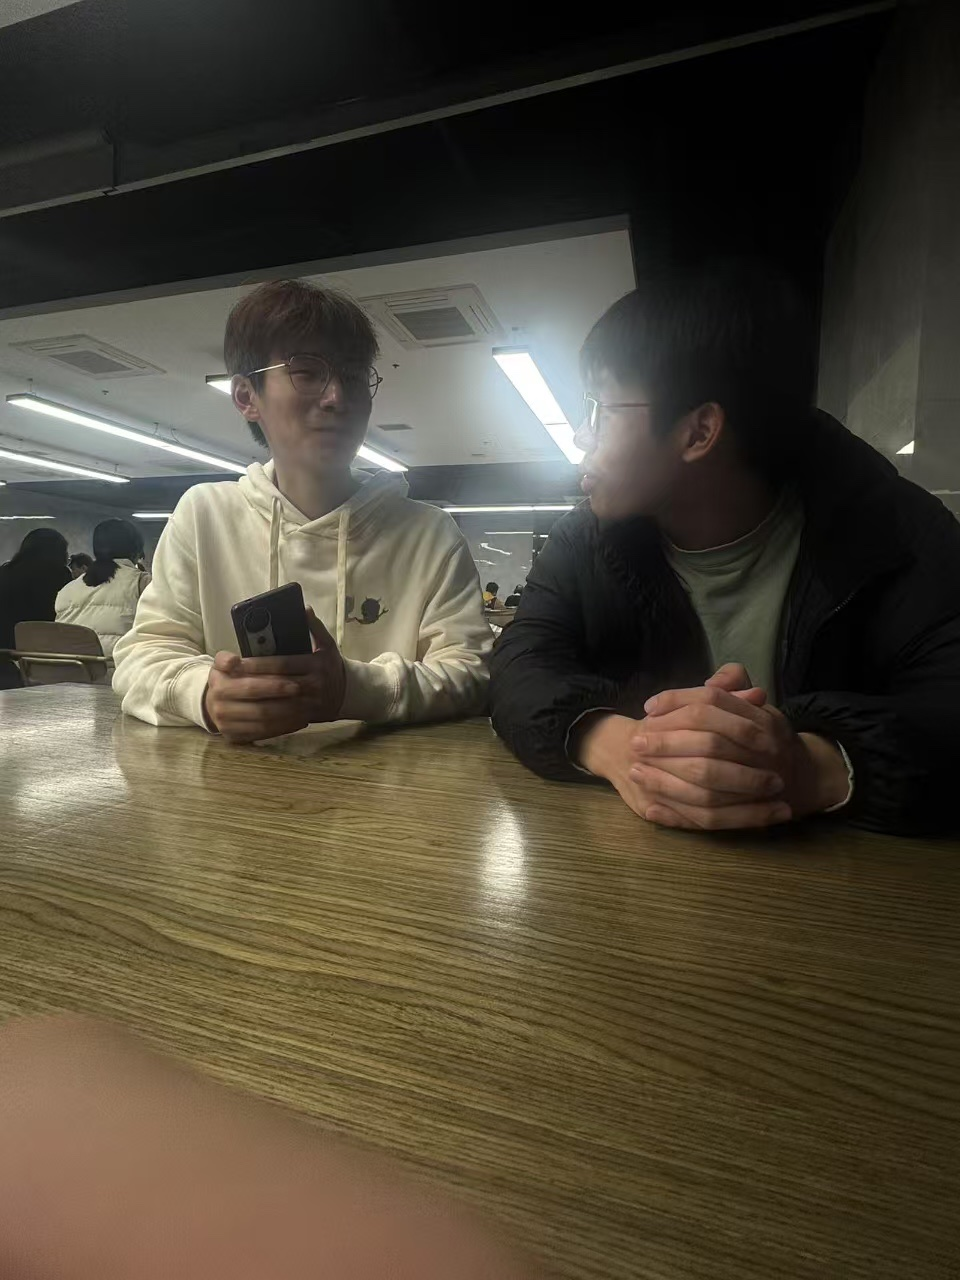
\includegraphics[width=\textwidth]{./resource/采访照片.JPG}
    \caption{线下采访照片}
\end{figure}